

\subsection{Rango de tiempo}
\begin{table}[H]
\centering
\begin{tabular}{c|c|c}
Inicio & 1388628499 & 2 January 2014 \\ \hline
Final  & 1550534100 & 18 February 2019 \\
\end{tabular}
\end{table}

\subsection{Tasa de eventos}

\begin{figure}[H]
	\centering
	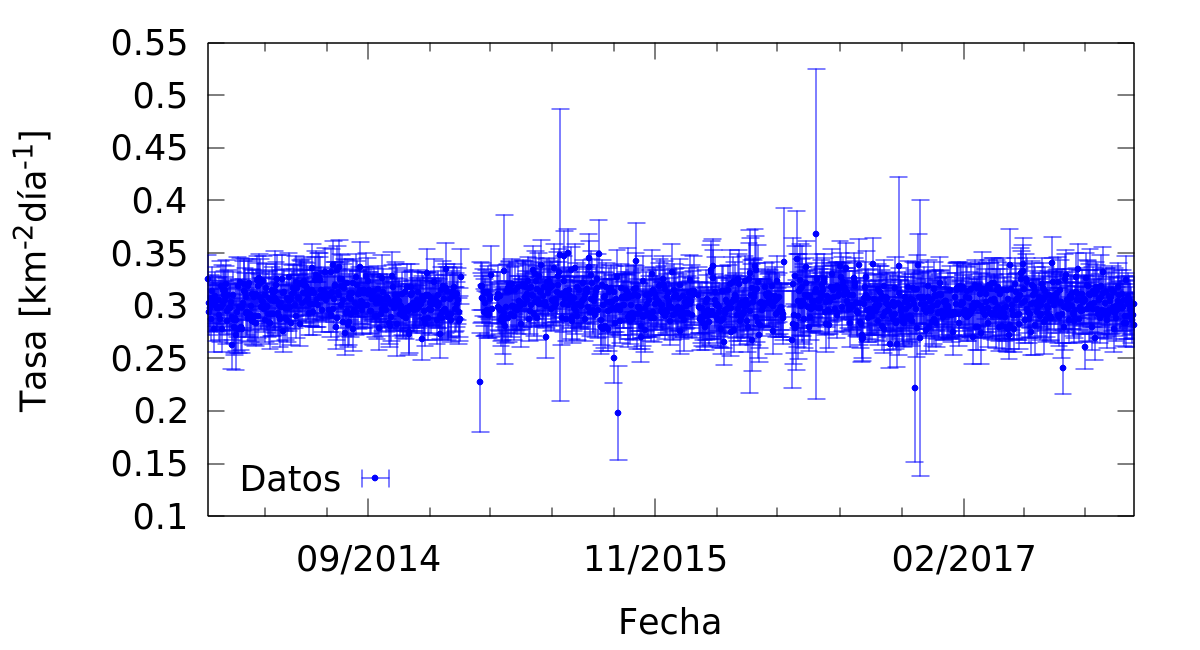
\includegraphics[width=0.5\textwidth]{rate_1_EeV.png}
	\caption{Tasa de eventos para eventos por encima de 1 EeV.}
\end{figure}

Antes del 2 de Enero del 2014, se tenía una tasa por debajo de la media de los siguientes años.

La cantidad de hexágonos 6T5 durante el periodo mencionado arriba evolucionó como se muestra  en la figura que sigue


\begin{figure}[H]
	\centering
	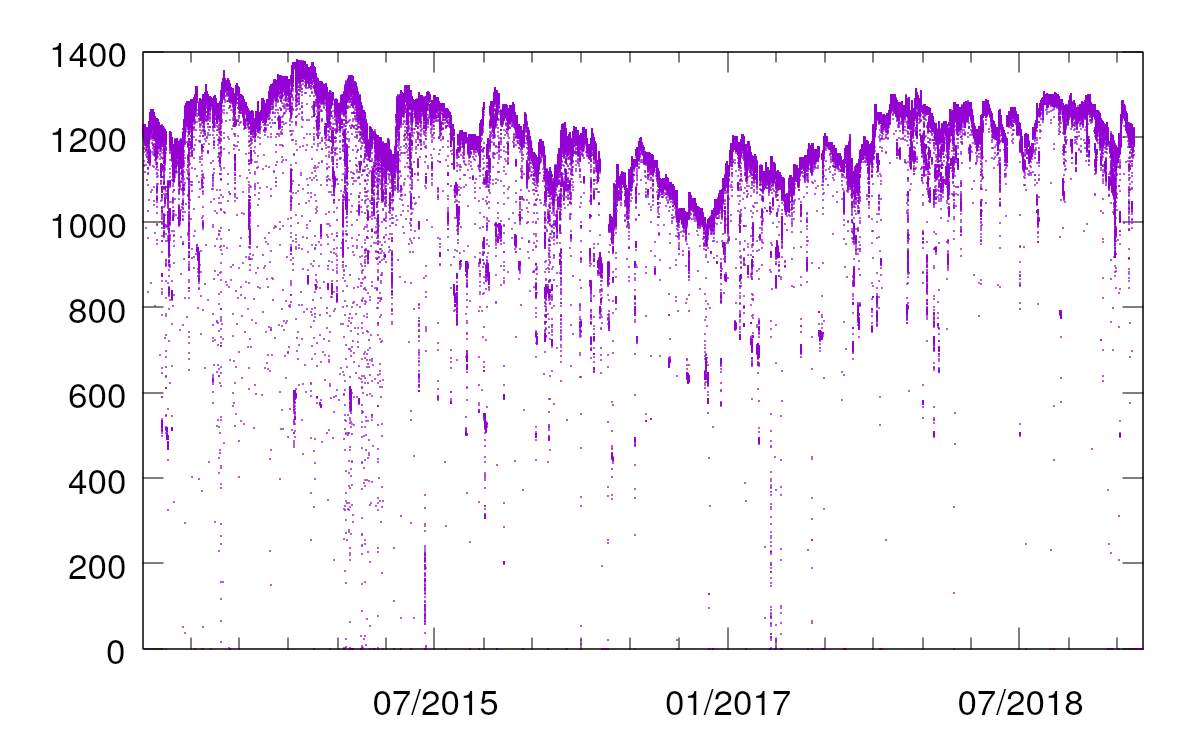
\includegraphics[width=0.5\textwidth]{hex_rango_corto.png}
	\caption{Hexágonos}
\end{figure}


\subsection{Párametros del clima}

\begin{figure}[H]
	\centering
	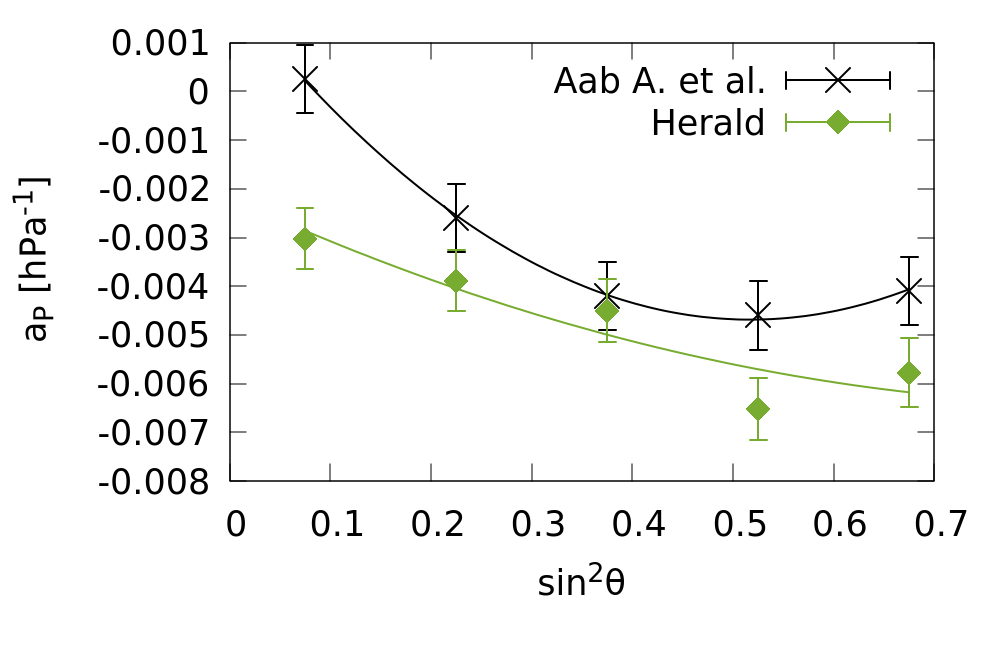
\includegraphics[width=0.5\textwidth]{ap.png}
\end{figure}


\begin{figure}[H]
	\centering
	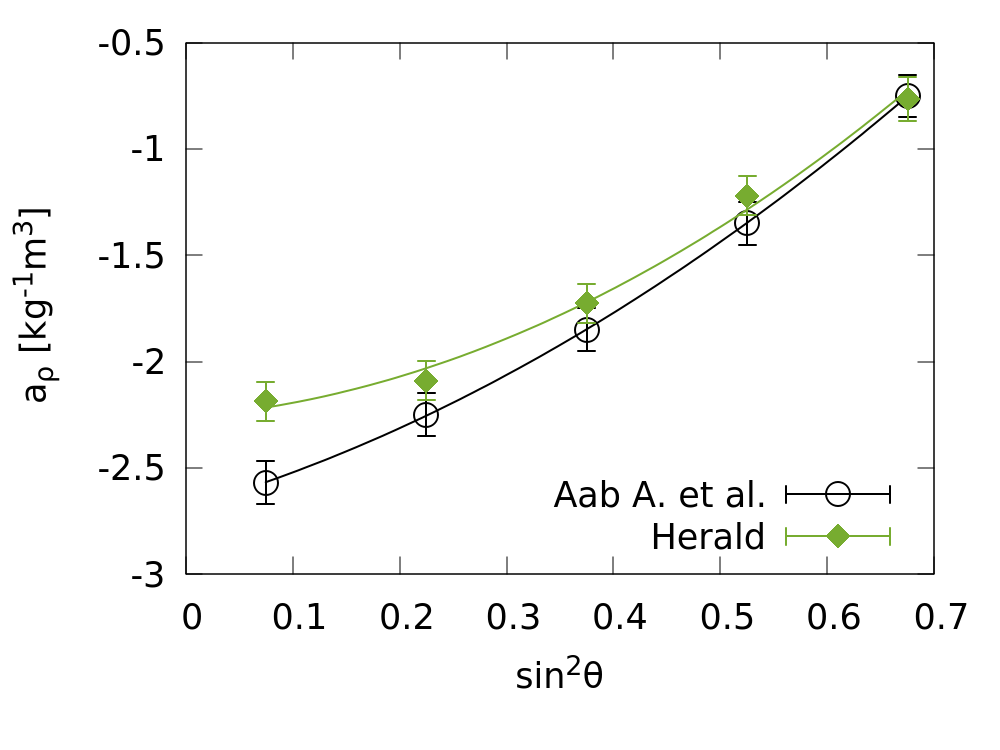
\includegraphics[width=0.5\textwidth]{arho.png}
\end{figure}


\begin{figure}[H]
	\centering
	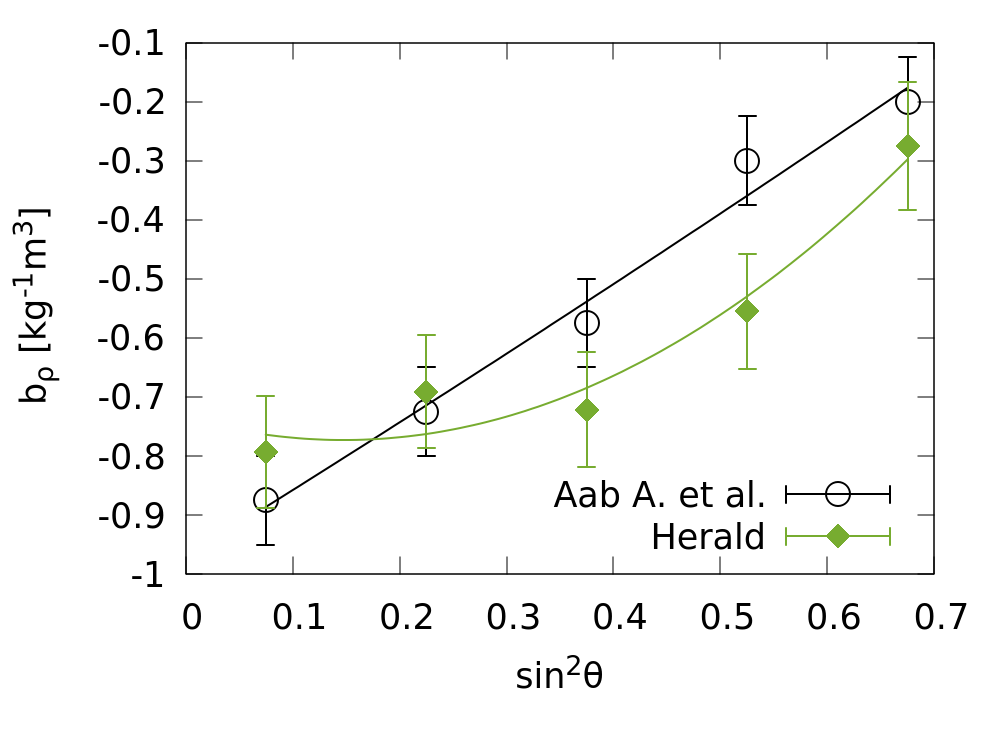
\includegraphics[width=0.5\textwidth]{brho.png}
\end{figure}




Considerando una cuádrica para el ajuste de la curva, se obtiene los parámetros de la siguiente table
\begin{table}[H]
\centering
\begin{tabular}{c|c|c|c}
		 	& $a_P$ 	&  $a_\rho$  & $ b_\rho$ \\ \hline
$c_0$ 		& -0.002(1) & 	-2.2(1)	 &	-0.74(9)\\ \hline
$c_1$ 		& -0.009(6)	& 	 0.4(6)	 &	-0.0(6)\\ \hline
$c_2$ 		&  0.00(9) 	& 	 2.7(8)  &	 1.7(7)\\ \hline
\end{tabular}
\end{table}


\subsection{Anisotropía en el rango 1-2 EeV}

\begin{figure}[htbp]
	\centering
	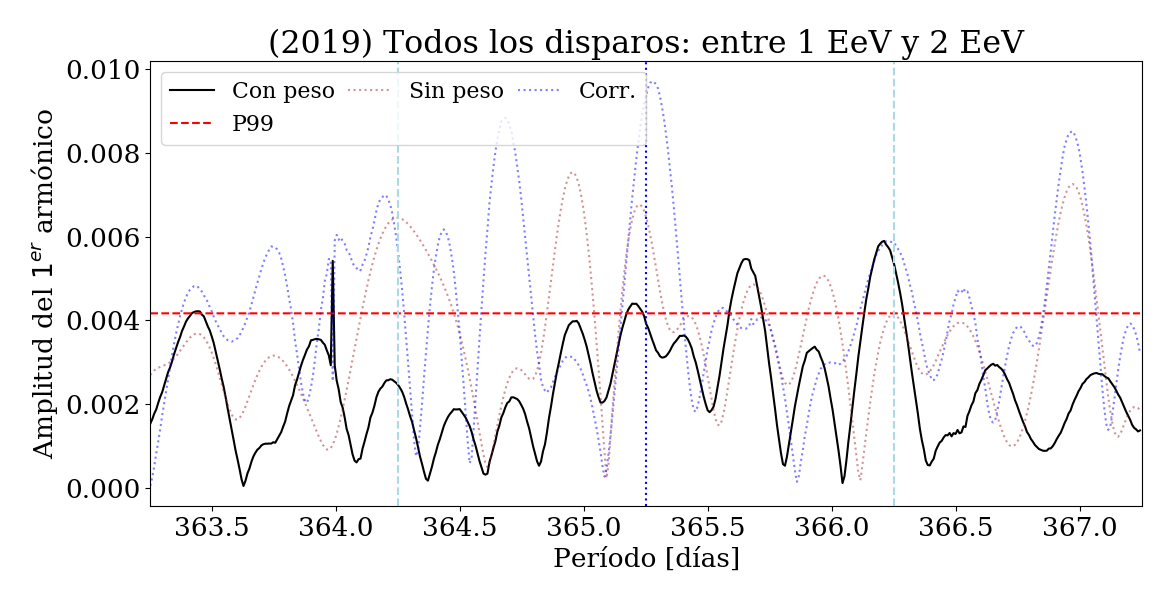
\includegraphics[width=0.5\textwidth]{ani_corr.png}
\end{figure}
